\section{Experiment 1}\label{sec:experiment-1}
%Needs an introduction to the experiment, and why it is relevant to the problem statement.
% relevance to problem anal. and introduction (why is this relavant)
The problem statement \ref{sec:problem-statement} proposes the investigation of the impact of dimensionality reduction on a chosen dataset, specifically comparing linear and nonlinear methods. This experiment will compare the selected dimensionality reduction methods in their optimal configurations on the chosen \gls{mnist} dataset. The objective is to determine the optimal configuration for each method, allowing for a fair comparison based on the same number of samples. The results of this experiment will provide insight into the impact of dimensionality reduction on machine learning models when applied in tandem.

\subsection{Rules and overview of experiment}\label{subsec:experiment-1-rules}
% Rules and what have we done, how do we evaluate (write about specs here)
The dimensionality reduction methods used in the experiment were \gls{svm}, \gls{pca}, \gls{lda}, \gls{kpca}, and \gls{isomap}. The baseline \gls{svm} \gls{ml} model was also used without any dimensionality reduction. Each method was first cross-validated, finding the best hyperparameters for 15000 samples. Every method was tested with the same number of components. Besides \gls{lda}, it can only use up to 9 components. Then some of the methods were cross-validated again with 60000 samples to find how the methods performed with more data; the same components were still used. The methods tested on 60000 samples were the baseline \gls{svm}, \gls{pca}, and \gls{lda}, as the computer used in the experiment could not handle \gls{kpca} and \gls{isomap} with 60000 samples of data. The configurations used for each are shown in Table \ref{tab:best-configuration}.

\begin{table}[htb!]   
    \centering
    \begin{tabular}{lrlll}
        \toprule
        method & components & C & parameter & parameter\\
        \midrule
        SVM-15 & 784 & C = 0.01 &  \\
        SVM-60 & 784 & C = 0.01 &  \\
        LDA-15 & 9 & C = 0.1 &  \\
        LDA-60 & 9 & C = 1.0 &  \\
        PCA-15 & 49 & C = 0.01 &  \\
        PCA-60 & 49 & C = 0.1 &   \\
        KPCA-15 & 49 & C = 1.0 & Gamma = 0.01 & Sigmoid \\
        ISOMAP-15 & 49 & C = 0.001 & neighbours = 5 \\
        \bottomrule
    \end{tabular}
    \caption{Best configuration for each method used for experiment-1, method-15 and method-60, means the method with 15 and 60 thousand samples.}
    \label{tab:best-configuration}
\end{table}

Every test in experiment 1 was made on the same computer, namely pc-2. See \autoref{tab:pc2-specs} for the specific specs for the computer used in the experiment. 

The experiment results are shown in \autoref{subsec:experiment-1-results}. The results are in the form of classification reports and confusion matrixes, which show the precision, recall, f1-score, support for each class, and the total accuracy for each method. The methods will be compared in accuracy, f1-score, and time fitting the data.

\subsection{Results}\label{subsec:experiment-1-results}
% Show results (desribe the most relavant results)
Below is shown the results for the methods. The results are in the form of classification reports, which show the precision, recall, f1-score, support for each class, and the total accuracy for each method. The methods will be compared in accuracy, f1-score, and time fitting the data. 

\begin{table}[htb!]
\centering
\begin{tabular}{lrrrr}
\toprule
 & precision & recall & f1-score & support \\
\midrule
0 & 94.7886 & 98.3673 & 96.5448 & 980 \\
1 & 96.3979 & 99.0308 & 97.6967 & 1135 \\
2 & 92.2488 & 93.4109 & 92.8262 & 1032 \\
3 & 90.8203 & 92.0792 & 91.4454 & 1010 \\
4 & 93.4739 & 94.8065 & 94.1355 & 982 \\
5 & 90.7940 & 88.4529 & 89.6082 & 892 \\
6 & 95.6705 & 94.5720 & 95.1181 & 958 \\
7 & 94.4828 & 93.2879 & 93.8815 & 1028 \\
8 & 93.1842 & 89.8357 & 91.4794 & 974 \\
9 & 92.8717 & 90.3865 & 91.6123 & 1009 \\
accuracy & & & 93.5400 & 10000 \\
macro avg & 93.4733 & 93.4230 & 93.4348 & 10000 \\
weighted avg & 93.5263 & 93.5400 & 93.5199 & 10000 \\
\bottomrule
\end{tabular}
\caption{Classification report for baseline\_svm\_15000}
\label{tab:classification-report-baseline_svm_15000}
\end{table}
 %37
\begin{figure}[htb!]
    \centering
    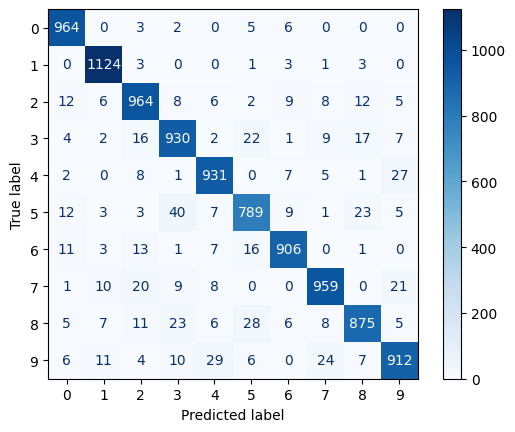
\includegraphics[width=0.8\textwidth]{figures/1-experiment/confusion_matrix_baseline_svm_15000.png}
    \caption{Confusion matrix for baseline SVM with 15000 samples.}
    \label{fig:confusion-matrix-baseline_svm_15000}
\end{figure}
\subsubsection{\gls{svm} with 15000 samples}\label{subsubsec:experiment-1-results-svm-15000}
Table \ref{tab:classification-report-baseline_svm_15000} shows the accuracy for \gls{svm} without any dimensionality reduction with 15000 samples. The accuracy is 93.54\%, and it takes 37 seconds to train the model. \autoref{fig:confusion-matrix-baseline_svm_15000} shows \gls{svm} is best at recognizing zeros and one's in pictures, as the model has the f1-score in these classes, with the scores 96.5\% and 97.7\%. The model has some trouble recognizing fives, eights, and threes, as these are the lowest scoring in the f1-score for all the classes, with five being 89.6\%, eight being 91.5\%, and three being 91.4\%. With an average f1-score of 93.43\%, the baseline \gls{svm} with 15000 samples is a good model. 

\subsubsection{\gls{svm} with 60000 samples}\label{subsubsec:experiment-1-results-svm-60000}
\begin{table}[htb!]
\centering
\begin{tabular}{lrrrr}
    \toprule
    & precision & recall & f1-score & support \\
    \midrule
    0 & 96.0278 & 98.6735 & 97.3327 & 980 \\
    1 & 97.3958 & 98.8546 & 98.1198 & 1135 \\
    2 & 93.6538 & 94.3798 & 94.0154 & 1032 \\
    3 & 91.6587 & 94.6535 & 93.1320 & 1010 \\
    4 & 93.8124 & 95.7230 & 94.7581 & 982 \\
    5 & 92.4138 & 90.1345 & 91.2599 & 892 \\
    6 & 96.2105 & 95.4071 & 95.8071 & 958 \\
    7 & 95.6262 & 93.5798 & 94.5919 & 1028 \\
    8 & 93.4668 & 91.0678 & 92.2517 & 974 \\
    9 & 94.8012 & 92.1705 & 93.4673 & 1009 \\
    accuracy & & & 94.5600 & 10000\\
    macro avg & 94.5067 & 94.4644 & 94.4736 & 10000 \\
    weighted avg & 94.5599 & 94.5600 & 94.5481 & 10000 \\
    \bottomrule
\end{tabular}
\caption{Classification report for baseline\_svm\_60000}
\label{tab:classification-report-baseline_svm_60000}
\end{table}
 %378
% \begin{figure}[htb!]
%     \centering
%     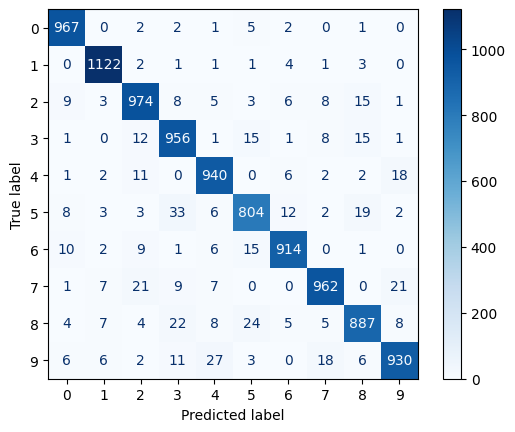
\includegraphics[width=0.8\textwidth]{figures/1-experiment/confusion_matrix_baseline_svm_60000.png}
%     \caption{Confusion matrix for baseline SVM with 60000 samples.}
%     \label{fig:confusion-matrix-baseline_svm_60000}
% \end{figure}
Table \ref{tab:classification-report-baseline_svm_60000} shows the accuracy for \gls{svm} without any dimensionality reduction with 60000 samples. The accuracy is 94.56\% for 60000 samples, and it takes 378 seconds to train the model, which is 6 minutes and 16 seconds. The \gls{svm} model is best at recognizing zeros and ones in pictures, as the model has the f1-score in these classes, with scores of 97.3\% and 98.1\%. The model has some trouble recognizing fives, eights, and threes, as these are the lowest scoring in the f1-score for all the classes, with five being 91.2\%, eight being 92.3\%, and three being 93.1\%. With an average f1-score of 94.47\%, the baseline \gls{svm} with 15000 samples is a good model that uses a significant amount of time.

\subsubsection{\gls{lda} with 15000 samples}\label{subsubsec:experiment-1-results-lda-15000}
\begin{table}[htb!]
\centering
\begin{tabular}{lrrrr}
    \toprule
    & precision & recall & f1-score & support \\
\midrule
0 & 93.1238 & 96.7347 & 94.8949 & 980 \\
1 & 94.3869 & 96.2996 & 95.3336 & 1135 \\
2 & 89.2246 & 85.8527 & 87.5062 & 1032 \\
3 & 85.1781 & 87.6238 & 86.3836 & 1010 \\
4 & 86.9650 & 91.0387 & 88.9552 & 982 \\
5 & 83.6549 & 82.6233 & 83.1359 & 892 \\
6 & 92.1466 & 91.8580 & 92.0021 & 958 \\
7 & 90.3353 & 89.1051 & 89.7160 & 1028 \\
8 & 83.2804 & 80.8008 & 82.0219 & 974 \\
9 & 87.7193 & 84.2418 & 85.9454 & 1009 \\
accuracy & & & 88.7600 & 10000 \\
macro avg & 88.6015 & 88.6178 & 88.5895 & 10000 \\
weighted avg & 88.7285 & 88.7600 & 88.7240 & 10000 \\
\bottomrule
\end{tabular}
\caption{Classification report for lda svm 15000}
\label{tab:classification-report-lda_svm_15000}
\end{table}
 %7
\begin{figure}[htb!]
    \centering
    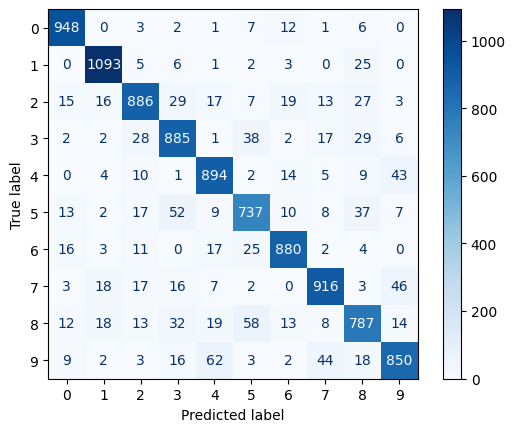
\includegraphics[width=0.8\textwidth]{figures/1-experiment/confusion_matrix_lda_svm_15000.png}
    \caption{Confusion matrix for LDA with 15000 samples.}
    \label{fig:confusion-matrix-lda-15000}
\end{figure}
Table \ref{tab:classification-report-lda_svm_15000} shows the accuracy for \gls{svm} with \gls{lda} as dimensionality reduction with 15000 samples. The accuracy is 88.76\% for 15000 samples, and it takes 7 seconds to train the model. \autoref{fig:confusion-matrix-lda-15000} \gls{svm} model is best at recognizing zeros and ones in pictures, as the model has the f1-score in these classes, with scores of 94.9\% and 95.3\%. The model has some trouble recognizing fives, eights, and nines, as these are the lowest scoring in the f1-score for all the classes, with five being 83.1\%, eight being 82.0\%, and three being 85.9\%. With an average f1-score of 88.59\%, the baseline \gls{svm}with 15000 samples is a worse model but is much faster than simply using \gls{svm}.
\subsubsection{\gls{lda} with 60000 samples}\label{subsubsec:experiment-1-results-lda-60000}
\begin{table}[htb!]
\centering
\begin{tabular}{lrrrr}
    \toprule
    & precision & recall & f1-score & support \\
    \midrule
0 & 93.1953 & 96.4286 & 94.7844 & 980 \\
1 & 94.7232 & 96.4758 & 95.5914 & 1135 \\
2 & 90.0398 & 87.5969 & 88.8016 & 1032 \\
3 & 85.9804 & 86.8317 & 86.4039 & 1010 \\
4 & 88.0929 & 92.6680 & 90.3226 & 982 \\
5 & 84.4318 & 83.2960 & 83.8600 & 892 \\
6 & 91.0387 & 93.3194 & 92.1649 & 958 \\
7 & 90.7093 & 88.3268 & 89.5022 & 1028 \\
8 & 84.9520 & 81.7248 & 83.3072 & 974 \\
9 & 88.4892 & 85.3320 & 86.8819 & 1009 \\
accuracy & & & 89.3300 & 10000 \\
macro avg & 89.1653 & 89.2000 & 89.1620 & 10000 \\
weighted avg & 89.2917 & 89.3300 & 89.2903 & 10000 \\
\bottomrule
\end{tabular}
\caption{Classification report for lda svm 60000}
\label{tab:classification-report-lda_svm_60000}
\end{table}
 %58
% \begin{figure}[htb!]
%     \centering
%     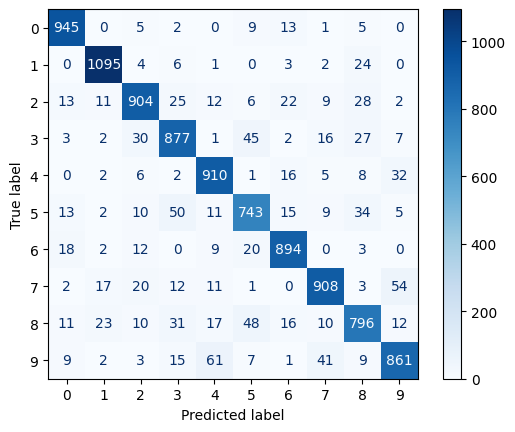
\includegraphics[width=0.8\textwidth]{figures/1-experiment/confusion_matrix_lda_svm_60000.png}
%     \caption{Confusion matrix for LDA with 60000 samples.}
%     \label{fig:confusion-matrix-lda-60000}
% \end{figure}
Table \ref{tab:classification-report-lda_svm_60000} shows the accuracy for \gls{svm} with \gls{lda} as dimensionality reduction with 60000 samples. The accuracy is 89.33\% for 60000 samples, and it takes 58 seconds to train the model. The \gls{svm} model is best at recognizing zeros and ones in pictures, as the model has the f1-score in these classes, with scores of 94.8\% and 95.6\%. The model has some trouble recognizing fives, eights, and threes, as these are the lowest scoring in the f1-score for all the classes, with five being 83.9\%, eight being 83.3\%, and three being 86.4\%. \gls{svm} using \gls{pca} as the dimensionality reduction method has an average f1-score of 89.16\%.

\subsubsection{\gls{pca} with 15000 samples}\label{subsubsec:experiment-1-results-pca-15000}
\begin{table}[htb!]
\centering
\caption{Classification report for pca_svm_15000}
\label{tab:classification-report-pca_svm_15000}
\begin{tabular}{lrrrr}
\toprule
 & precision & recall & f1-score & support \\
\midrule
0 & 0.944773 & 0.977551 & 0.960883 & 980.000000 \\
1 & 0.967938 & 0.984141 & 0.975972 & 1135.000000 \\
2 & 0.904306 & 0.915698 & 0.909966 & 1032.000000 \\
3 & 0.897335 & 0.900000 & 0.898665 & 1010.000000 \\
4 & 0.916914 & 0.943992 & 0.930256 & 982.000000 \\
5 & 0.889143 & 0.872197 & 0.880589 & 892.000000 \\
6 & 0.951832 & 0.948852 & 0.950340 & 958.000000 \\
7 & 0.923002 & 0.921206 & 0.922103 & 1028.000000 \\
8 & 0.904963 & 0.879877 & 0.892244 & 974.000000 \\
9 & 0.927083 & 0.882061 & 0.904012 & 1009.000000 \\
accuracy & 0.923700 & 0.923700 & 0.923700 & 0.923700 \\
macro avg & 0.922729 & 0.922558 & 0.922503 & 10000.000000 \\
weighted avg & 0.923513 & 0.923700 & 0.923467 & 10000.000000 \\
\bottomrule
\end{tabular}
\end{table}
 %10
\begin{figure}[htb!]
    \centering
    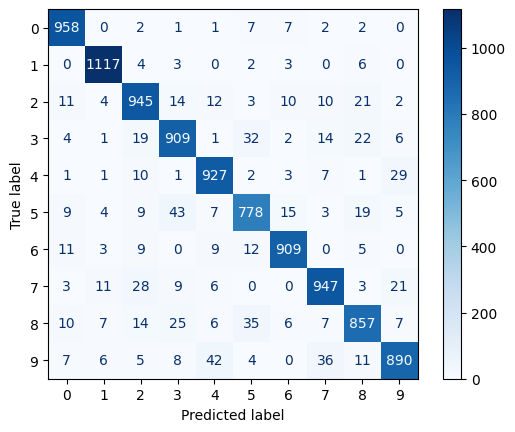
\includegraphics[width=0.8\textwidth]{figures/1-experiment/confusion_matrix_pca_svm_15000.png}
    \caption{Confusion matrix for PCA with 15000 samples.}
    \label{fig:confusion-matrix-pca-15000}
\end{figure}
Table \ref{tab:classification-report-pca_svm_15000} shows the accuracy for \gls{svm} with \gls{pca} as dimensionality reduction with 15000 samples. The accuracy is 92.37\% for 15000 samples, and it takes 10 seconds to train the model. \autoref{fig:confusion-matrix-pca-15000} \gls{svm} model is best at recognizing zeros and ones in pictures, as the model has the f1-score in these classes, with scores of 96.1\% and 97.6\%. The model has some trouble recognizing fives, eights, and threes, as these are the lowest scoring in the f1-score for all the classes, with five being 88.1\%, eight being 89.2\%, and three being 89.9\%. \gls{svm} using \gls{pca} as the dimensionality reduction method has an average f1-score of 92.25\%.

\subsubsection{\gls{pca} with 60000 samples}\label{subsubsec:experiment-1-results-pca-60000}
\begin{table}[htb!]
\centering
\begin{tabular}{lrrrr}
    \toprule
    & precision & recall & f1-score & support \\
    \midrule
    0 & 94.8768 & 98.2653 & 96.5414 & 980 \\
    1 & 96.7993 & 98.5903 & 97.6866 & 1135 \\
    2 & 92.3301 & 92.1512 & 92.2405 & 1032 \\
    3 & 88.9952 & 92.0792 & 90.5109 & 1010 \\
    4 & 92.3153 & 95.4175 & 93.8408 & 982 \\
    5 & 90.4157 & 87.7803 & 89.0785 & 892 \\
    6 & 95.7336 & 96.0334 & 95.8833 & 958 \\
    7 & 94.3620 & 92.8016 & 93.5753 & 1028 \\
    8 & 92.2340 & 89.0144 & 90.5956 & 974 \\
    9 & 93.7565 & 89.2963 & 91.4721 & 1009 \\
    accuracy &  & & 93.2500 & 10000\\
    macro avg & 93.1819 & 93.1429 & 93.1425 & 10000 \\
    weighted avg & 93.2474 & 93.2500 & 93.2290 & 10000 \\
\bottomrule
\end{tabular}
\caption{Classification report for pca svm 60000}
\label{tab:classification-report-pca_svm_60000}
\end{table}
 %97
% \begin{figure}[htb!]
%     \centering
%     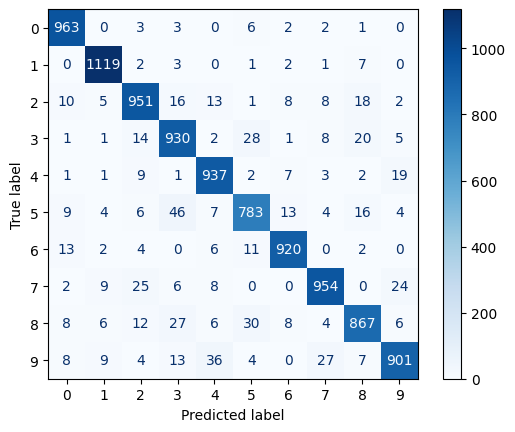
\includegraphics[width=0.8\textwidth]{figures/1-experiment/confusion_matrix_pca_svm_60000.png}
%     \caption{Confusion matrix for PCA with 60000 samples.}
%     \label{fig:confusion-matrix-pca-60000}
% \end{figure}
Table \ref{tab:classification-report-pca_svm_60000} shows the accuracy for \gls{svm} with \gls{pca} as dimensionality reduction with 60000 samples. The accuracy is 93.25\% for 60000 samples, and it takes 97 seconds to train the model, which is 1 minute and 37 seconds. The \gls{svm} model is best at recognizing zeros and ones in pictures, as the model has the f1-score in these classes, with scores of 96.5\% and 97.7\%. The model has some trouble recognizing fives, eights, and threes, as these are the lowest scoring in the f1-score for all the classes, with five being 89.1\%, eight being 90.6\%, and three being 90.5\%. \gls{svm} using \gls{pca} as the dimensionality reduction method has an average f1-score of 93.14\%.

\subsubsection{\gls{kpca} with 15000 samples}\label{subsubsec:experiment-1-results-kernel_pca-15000}
\begin{table}[htb!]
\centering
\caption{Classification report for kernel_pca_svm_15000}
\label{tab:classification-report-kernel_pca_svm_15000}
\begin{tabular}{lrrrr}
\toprule
 & precision & recall & f1-score & support \\
\midrule
0 & 0.943137 & 0.981633 & 0.962000 & 980.000000 \\
1 & 0.968858 & 0.986784 & 0.977739 & 1135.000000 \\
2 & 0.911005 & 0.922481 & 0.916707 & 1032.000000 \\
3 & 0.893175 & 0.894059 & 0.893617 & 1010.000000 \\
4 & 0.915842 & 0.941955 & 0.928715 & 982.000000 \\
5 & 0.881609 & 0.859865 & 0.870602 & 892.000000 \\
6 & 0.937824 & 0.944676 & 0.941238 & 958.000000 \\
7 & 0.929342 & 0.921206 & 0.925256 & 1028.000000 \\
8 & 0.927039 & 0.887064 & 0.906611 & 974.000000 \\
9 & 0.916667 & 0.883053 & 0.899546 & 1009.000000 \\
accuracy & 0.923600 & 0.923600 & 0.923600 & 0.923600 \\
macro avg & 0.922450 & 0.922278 & 0.922203 & 10000.000000 \\
weighted avg & 0.923360 & 0.923600 & 0.923321 & 10000.000000 \\
\bottomrule
\end{tabular}
\end{table}
 %92
\begin{figure}[htb!]
    \centering
    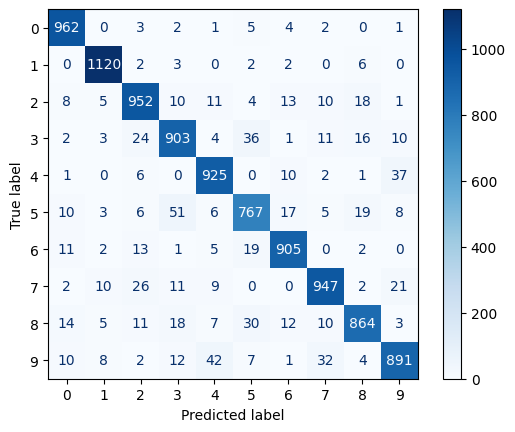
\includegraphics[width=0.8\textwidth]{figures/1-experiment/confusion_matrix_kernel_pca_svm_15000.png}
    \caption{Confusion matrix for kernel PCA with 15000 samples.}
    \label{fig:confusion-matrix-kpca-15000}
\end{figure}
Table \ref{tab:classification-report-kernel_pca_svm_15000} shows the accuracy for \gls{svm} with \gls{kpca} as dimensionality reduction with 15000 samples. The accuracy is 92.36\% for 15000 samples, and it takes 92 seconds to train the model, which is 1 minute and 32 seconds. \autoref{fig:confusion-matrix-kpca-15000} \gls{svm} model is best at recognizing zeros and ones in pictures, as the model has the f1-score in these classes, with scores of 96.2\% and 97.8\%. The model has trouble recognizing fives, nines, and threes, as these are the lowest scores in the f1-score for all the classes, with five being 87.1\%, nine being 90.0\%, and three being 89.4\%. \gls{svm} using \gls{kpca} as the dimensionality reduction method has an average f1-score of 92.22\%.

\subsubsection{\gls{isomap} with 15000 samples}\label{subsubsec:experiment-1-results-isomap-15000}
\begin{table}[htb!]
\centering
\begin{tabular}{lrrrr}
    \toprule
 & precision & recall & f1-score & support \\
\midrule
0 & 93.1507 & 97.1429 & 95.1049 & 980 \\
1 & 94.2953 & 99.0308 & 96.6051 & 1135 \\
2 & 92.1509 & 87.5969 & 89.8162 & 1032 \\
3 & 88.2579 & 90.7921 & 89.5071 & 1010 \\
4 & 91.5725 & 90.7332 & 91.1509 & 982 \\
5 & 87.7232 & 88.1166 & 87.9195 & 892 \\
6 & 95.1426 & 94.0501 & 94.5932 & 958 \\
7 & 88.5375 & 87.1595 & 87.8431 & 1028 \\
8 & 89.7297 & 85.2156 & 87.4144 & 974 \\
9 & 84.8963 & 85.2329 & 85.0643 & 1009 \\
accuracy & & & 90.6100 & 10000\\
macro avg & 90.5457 & 90.5071 & 90.5019 & 10000 \\
weighted avg & 90.5947 & 90.6100 & 90.5771 & 10000 \\
\bottomrule
\end{tabular}
\caption{Classification report for isomap\_svm\_15000}
\label{tab:classification-report-isomap_svm_15000}
\end{table}
 %165
\begin{figure}[htb!]
    \centering
    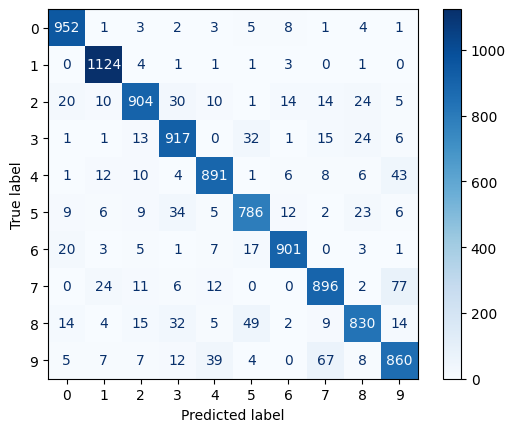
\includegraphics[width=0.8\textwidth]{figures/1-experiment/confusion_matrix_isomap_svm_15000.png}
    \caption{Confusion matrix for ISOMAP with 15000 samples.}
    \label{fig:confusion-matrix-isomap-15000}
\end{figure}
Table \ref{tab:classification-report-isomap_svm_15000} shows the accuracy for \gls{svm} with \gls{isomap} as dimensionality reduction with 15000 samples. The accuracy is 90.61\% for 15000 samples, and it takes 165 seconds to train the model, which is 2 minutes and 45 seconds. \autoref{fig:confusion-matrix-isomap-15000} \gls{svm} model is best at recognizing zeros and ones in pictures, as the model has the f1-score in these classes, with scores of 95.1\% and 96.6\%. The model has trouble recognizing sevens, eights, and nines, as these are the lowest scoring in the f1-score for all the classes, with seven being 87.8\%, eight being 87.4\%, and three being 85.1\%. \gls{svm} using \gls{isomap} as the dimensionality reduction method has an average f1-score of 90.50\%.

\subsection{Discussion experiment 1}\label{sec:discussion-experiment-1}
% discus the results to the problem statement
Comparing the results from experiment 1 is done in two comparisons; the first comparison is between the accuracy and time for the different dimensionality reduction methods. The second comparison is between the f1-scores for the different dimensionality reduction methods and what numbers the models are worst at recognizing. 

\subsubsection{Accuracy and time}\label{subsec:discussion-experiment-1-accuracy}
All experiments done is displayed in Table \ref{tab:discussion-experiment-1-accuracy}, it shows the accuracy for all the different models and the time taken.

\begin{table}
    \centering
    \begin{tabular}{lll}
        \hline
        Reduction method & Accuracy & Time \\
        \hline
        \gls{svm}-15 & 93.54\% & 37 seconds \\
        \gls{lda}-15 & 88.76\% & 7 seconds \\
        \gls{pca}-15 & 92.37\% & 10 seconds \\
        \gls{kpca}15 & 92.36\% & 92 seconds \\
        \gls{isomap}-15 & 90.61\% & 165 seconds \\
        \hline
        \gls{svm}-60 & 94.54\% & 378 seconds \\
        \gls{lda}-60 & 89.33\% & 58 seconds \\
        \gls{pca}-60 & 93.25\% & 97 seconds \\
        \hline
    \end{tabular}
    \caption{Accuracy and time for the different dimensionality reduction methods,  method-15 and method-60, means the method with 15 and 60 thousand samples.}
    \label{tab:discussion-experiment-1-accuracy}
    \end{table}
In \autoref{fig:discussion-experiment-1-plot} show the comparison between the methods with 15000 samples. The baseline \gls{svm}, on 15000 samples, has an accuracy of 93.54\%, and it takes 37 seconds to train the model. The baseline \gls{svm} can also be suitable to compare the other models, as it is an excellent model to hold as the baseline.

The accuracy increases by 1\% when using 45000 more samples, which is a slight difference. One thing to note is that it takes 37 seconds to train the model on 15000 samples and 378 seconds to train the model on 60000 samples. This means that the time it takes to train the model grows 921,62\% by using 45000 more examples of data. This is a big difference in time but a slight difference in accuracy.

\begin{figure}[htb!]
    \centering
    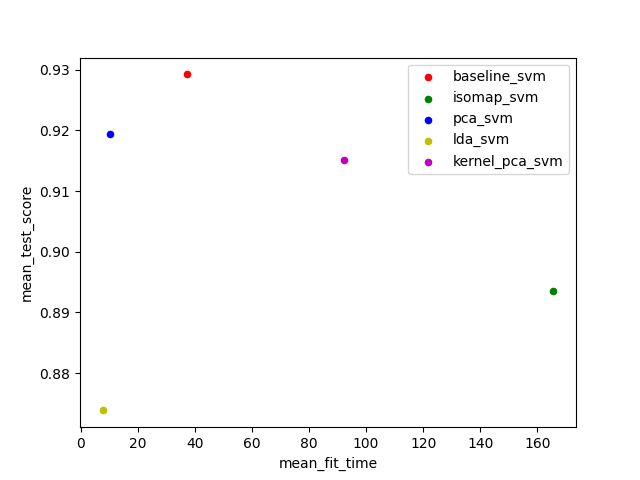
\includegraphics[width=0.8\textwidth]{figures/1-experiment/experiment1_plot.png}
    \caption{graph of time(in seconds) and accuracy(in percentage) for different dimensionality reduction methods}
    \label{fig:discussion-experiment-1-plot}
\end{figure}

When using \gls{lda} on 15000 samples, the accuracy falls to 88.76\%, but it only takes 7 seconds to train the model. \gls{lda} has a swift training time but low accuracy, but one thing to note, is that the maximum number of dimensions \gls{lda} can reduce to is 9 in this context. Therefore, the scores for \gls{lda} are worse than any dimensionality reduction method used. As the other methods use 49 dimensions to reduce the data, which is much higher than 9, it makes sense that the accuracy is higher than \gls{lda}. \gls{lda} only takes 7 seconds to train the model, so it is an excellent method to use if one wants a fast model with lower accuracy by comparing the other methods with more dimensions. 

When using 60000 samples, the accuracy is 89.33\%, and it takes 58 seconds to train the model. This means that the time it takes to train the model grows 728,57\% by using 45000 more examples of data. This is a big difference in time but a slight difference in accuracy; however, \gls{lda} is the fastest method, with lower accuracy than other methods. By using \gls{lda}, the model is faster but comes with the cost of lower accuracy.

When using \gls{pca} on 15000 samples, the accuracy is 92.37\%, and it takes 10 seconds to train the model, which is faster than the baseline \gls{svm} alone but still slower than \gls{lda} with the same amount of samples. When using 60000 samples, the accuracy is 93.25\%, and it takes 97 seconds to train the model. This means that the time it takes to train the model grows by 870\% by using 45000 more data samples. \gls{pca} has a lower accuracy than the baseline \gls{svm}. It is still faster than \gls{svm} alone but slower than \gls{lda}, making the model a good choice if one wants a faster model with slightly lower accuracy than the baseline \gls{svm}.

When using \gls{kpca} on 15000 samples, the accuracy is 92.36\%, and it takes 92 seconds to train the model. \gls{kpca} is slower than the baseline \gls{svm} and linear methods; this makes sense since nonlinear dimensionality methods can be heavier to compute. Nevertheless, \gls{kpca} scores the highest accuracy of all the dimensionality reduction methods used when using 15000 samples. If the computational cost is not an issue, \gls{kpca} is the best dimensionality reduction.

When using \gls{isomap} on 15000 samples, the accuracy is 90.61\%, and it takes 165 seconds to train the model. \gls{isomap} is slower than all the other dimensionality reduction methods and the baseline \gls{svm}. This makes sense since nonlinear dimensionality methods can be heavier to compute. However, \gls{isomap} scores the second lowest accuracy of all the dimensionality reduction methods used when using 15000 samples. So there are better dimensionality reduction methods than \gls{isomap} if one wants a fast model with high accuracy.

To conclude from this experiment, the baseline \gls{svm} is the best model to use if one wants a fast model with high accuracy. If one wants a faster model with lower accuracy, \gls{lda} is the best model to use. If one wants a model with high accuracy but slower than the baseline \gls{svm}, \gls{kpca} is the best model. If one wants a model with high accuracy but slower than the baseline \gls{svm}, \gls{isomap} is the best model. \gls{pca} is the best model if one wants a model with high accuracy and faster than the baseline SVM.

\subsubsection{F1-scores}\label{subsec:discussion-experiment-1-f1-score}
One thing to note is that the f1-score is the harmonic mean of precision and recall, which means that the f1-score is the average of the precision and recall. The f1-score is an excellent metric to use when the classes need to be balanced, as it is the average of precision and recall.
\begin{table}
    \centering
    \begin{tabular}{llrrr}
        \hline
        Reduction method & f1-score & worst score & 2. worst score & 3. worst score \\
        \hline
        \gls{svm}-15 & 93.43\% & 5 & 3 & 8 \\
        \gls{svm}-60 & 94.47\% & 5 & 8 & 3 \\
        \gls{lda}-15 & 88.59\% & 8 & 5 & 9 \\
        \gls{lda}-60 & 89.16\% & 8 & 5 & 3 \\
        \gls{pca}-15 & 92.25\% & 5 & 8 & 3 \\
        \gls{pca}-60 & 93.14\% & 5 & 3 & 8 \\
        \gls{kpca}-15 & 92.22\% & 5 & 3 & 9 \\
        \gls{isomap}-15 & 90.50\% & 9 & 8 & 7 \\
        \hline
    \end{tabular}
    \caption{F1-scores for the different dimensionality reduction methods.}
    \label{tab:discussion-experiment-1-f1-score}
    \end{table}
All experiments are displayed in Table \ref{tab:discussion-experiment-1-f1-score}, which shows the f1-score for the different models and the three worst classes for f1-scores.
In all experiments done, all of the models have a high f1-score, which means that the models are good at recognizing the numbers in the pictures. all models are best at recognizing zeros and ones in pictures. and good at recognizing four and sixes. When it comes to what the different models are bad at distinguishing, it is different for all. The most common number that the models are bad at recognizing is threes, fives, and eights, in a different order depending on the dimensionality reduction method used as these are the worst in \gls{svm} with both 15000 and 60000 samples, \gls{lda} with 60000 samples, \gls{pca} with 15000 samples and 60000 samples. \gls{isomap} is the only model that could be better at recognizing threes or fives, as it is terrible at sevens, eights, and nines. This can impact if one wants to use the model to find threes or fives; \gls{isomap} can be considered, as it is good at recognizing these numbers.

\gls{lda} with 15000 samples is interesting, as it needs to improve recognizing fives, eights, and nines. This is interesting as \gls{lda} with 60000 samples needs to improve recognizing threes, fives, and eights. This means \gls{lda} gets better at recognizing nines. This can be because more nines come into the dataset using 60000 samples, which makes \gls{lda} better at recognizing nines. 

In the occasions where there is more than one experiment done to the same method, the worst f1-scores for a class change, as seen in \gls{pca}, where at 15000 samples, the eights have the second worst f1-score, but at 60000 samples, the eights have the third worst f1-score. So the worst f1-scores for a class can change depending on the number of samples used.

To conclude this experiment, the models are good at recognizing the numbers in the pictures, but they are not perfect. The models are best at recognizing zeros and ones in pictures and recognizing four and sixes. When it comes to what the different models are bad at distinguishing, it is different for all. The most common number that the models are bad at recognizing is threes, fives, and eights, in a different order depending on the dimensionality reduction method used as these are the worst in \gls{svm} with both 15000 and 60000 samples, \gls{lda} with 60000 samples, \gls{pca} with 15000 samples and 60000 samples. \gls{isomap} is the only model that is not bad at recognizing threes or fives, as it is terrible at sevens, eights, and nines. This can have an impact if one wants to use the model to find threes or fives, \gls{isomap}P can be considered, as it is not bad at recognizing these numbers, but if one wants to use the model to find eights, then \gls{isomap} is not a good choice.

%intro
%presentation af de experimenter vi har valgt og hvorfor vi har valgt dem?
% experiment 1 exemple
%     detaljeret gennemgang af regler og evaluering
%     fremvisning af resultater
%     opsumering af resultater
%     diskussion af resultater og hvad der ellers var spændende evaluering af hvorfor det blev sådan.
%why this experiment was chosen
%look at f1-score and accuracy and time fitting the data